\documentclass{amsbook}

\usepackage{amssymb}
\usepackage{hyperref}
\usepackage{enumitem}
\usepackage{mathtools}
\usepackage{geometry}                % See geometry.pdf to learn the layout options. There are lots.
\usepackage{bm}
\geometry{a4paper}                   % ... or a4paper or a5paper or ... 

\newtheorem{theorem}{Theorem}[chapter]
\newtheorem{lemma}[theorem]{Lemma}

\theoremstyle{definition}
\newtheorem{definition}[theorem]{Definition}
\newtheorem{example}[theorem]{Example}
\newtheorem{xca}[theorem]{Exercise}

\theoremstyle{remark}
\newtheorem{remark}[theorem]{Remark}

\numberwithin{section}{chapter}
\numberwithin{equation}{chapter}

\begin{document}

\frontmatter

\title{Minqi's Solutions to the Problems of Peter J. Bickel and Kjell A. Doksum (2015), Mathematical Statistics: Basic Ideas and Selected Topics, Volume I (2nd Edition)}

\author{Minqi Pan\footnote{Website: http://www.minqi-pan.com}}

\date{\today}

\maketitle

\setcounter{page}{4}

\tableofcontents

\mainmatter

\chapter{Statistical Models, Goals, and Performance Criteria}

\section{Problem 1.1.1: Examples of Statistical Models}
Give a formal statement of the following models identifying the probability laws of the data and the parameter space. State whether the model in question is parametric or nonparametric.
\begin{enumerate}[label=(\alph*)]
\item A geologist measures the diameters of a large number $n$ of pebbles in an old stream bed.
Theoretical considerations lead him to believe that the logarithm of pebble diameter is normally distributed with mean $\mu$ and variance $\sigma$.
He wishes to use his observations to obtain some information about $\mu$ and $\sigma^2$
but has in advance no knowledge of the magnitudes of the two parameters.
\item A measuring instrument is being used to obtain $n$ independent determinations of a physical constant $\mu$.
Suppose that the measuring instrument is known to be biased to the positive side by $0.1$ units.
Assume that the errors are otherwise identically distributed normal random variables with known variance.
\item In part (b) suppose that the amount of bias is positive but unknown. Can you perceive any difficulties in making statements about $\mu$ for this model?
\item The number of eggs laid by an insect follows a Poisson distribution with unknown mean $\lambda$.
Once laid, each egg has an unknown chance $p$ of hatching and the hatching of one egg is independent of the hatching of the others.
An entomologist studies a set of $n$ such insects observing both the number of eggs laid and the number of eggs hatching for each nest.
\end{enumerate}
\begin{proof}[Answer]
\begin{enumerate}[label=(\alph*)]
\item Let sample space $\Omega$ be defined by\[
\Omega\equiv\{(P_1,\dots,P_n):P_i\text{ is a pebble of the old stream}\}.
\]Let $\mathbf{X}:\Omega\to\mathbb{R}^n$ be the random vector defined by\[
\begin{split}
\mathbf{X}&\equiv(X_1,\dots,X_n),\\
X_i(P_1,\dots,P_n)&\equiv\log(\text{diameter of }P_i).
\end{split}
\]We assume that $\mathbf{X}\sim P_{\mu,\sigma^2}$, where $P_{\mu,\sigma^2}$ is a probability distribution on $\mathbb{R}^n$ according to which $X_1,\dots,X_n$ are independent and identically distributed with a common $\mathcal{N}(\mu,\sigma^2)$ distribution. Let the parameter space $\Theta$ be defined by\[
\Theta\equiv\{(\mu,\sigma^2):\mu\in\mathbb{R},\sigma^2>0\}.
\]Finally, let model $\mathcal{P}$ be defined by\[
\mathcal{P}\equiv\{P_{\mu,\sigma^2}:(\mu,\sigma^2)\in\Theta\}.
\]$\mathcal{P}$ is parametric.
\item Let sample space $\Omega$ be defined by\[
\Omega\equiv\{(D_1,\dots,D_n)\in\mathbb{R}^n:D_i\text{ is a determination of the physical constant}\}.
\]Let $\mathbf{X}:\Omega\to\mathbb{R}^n$ be the random vector defined by\[
\begin{split}
\mathbf{X}&\equiv(X_1,\dots,X_n),\\
X_i(D_1,\dots,D_n)&\equiv D_i.
\end{split}
\]Let $\mathbf{Y}=(Y_1,\dots,Y_n):\Omega\to\mathbb{R}^n$ be the random vector defined by\[
\mathbf{Y}=\mathbf{X}-\mu.
\]We assume that $\mathbf{Y}\sim P_{\sigma_0^2}$, where $P_{\sigma_0^2}$ is a probability distribution on $\mathbb{R}^n$ according to which $Y_1,\dots,Y_n$ are independently and identically distributed with a common $\mathcal{N}(+0.1,\sigma_0^2)$ distribution, where $\sigma_0^2$ is the known variance. Therefore\[
X_i\sim\mathcal{N}(\mu+0.1,\sigma_0^2),\quad\forall i=1,\dots,n.
\]That is to say, $\mathbf{X}\sim P_{\mu+0.1}$, where $P_{\mu+0.1}$ is a probability distribution on $\mathbb{R}^n$ according to which $X_1,\dots,X_n$ are independent and identically distributed with a common $\mathcal{N}(\mu+0.1,\sigma_0^2)$ distribution. Let the parameter space $\Theta$ be defined by\[
\Theta\equiv\{\mu+0.1:\mu+0.1\in\mathbb{R}\}.
\]Finally, let model $\mathcal{P}$ be defined by\[
\mathcal{P}\equiv\{P_{\mu+0.1}:\mu+0.1\in\Theta\}.
\]$\mathcal{P}$ is parametric.
\item Yes. The difficulty is that we need one more parameter $\mu'$, and the parametrization becomes unidentifiable. Specifically, we need to assume that $\mathbf{Y}\sim P_{\mu',\sigma_0^2}$, where $P_{\mu',\sigma_0^2}$ is a probability distribution on $\mathbb{R}^n$ according to which $Y_1,\dots,Y_n$ are independently and identically distributed with a common $\mathcal{N}(\mu',\sigma_0^2)$ distribution. Therefore\[
X_i\sim\mathcal{N}(\mu+\mu',\sigma_0^2),\quad\forall i=1,\dots,n.
\]That is to say, $\mathbf{X}\sim P_{\mu,\mu'}$, where $P_{\mu,\mu'}$ is a probability distribution on $\mathbb{R}^n$ according to which $X_1,\dots,X_n$ are independent and identically distributed with a common $\mathcal{N}(\mu+\mu',\sigma_0^2)$ distribution. Let the parameter space $\Theta$ be defined by\[
\Theta\equiv\{(\mu,\mu'):\mu\in\mathbb{R},\mu'\in\mathbb{R}\}.
\]Finally, let model $\mathcal{P}$ be defined by\[
\mathcal{P}\equiv\{P_{\mu,\mu'}:(\mu,\mu')\in\Theta\}.
\]$\mathcal{P}$ is parametric.
\item Let sample space $\Omega$ be defined by\[
\Omega\equiv\{(N_1,\dots,N_n):N_i\text{ is a nest}\}.
\]Let $\mathbf{X}:\Omega\to\mathbb{R}^n$ be the random vector defined by\[
\begin{split}
\mathbf{X}&\equiv(X_1,\dots,X_n),\\
X_i(N_1,\dots,N_n)&\equiv\text{the number of eggs laid in }N_i.
\end{split}
\]Let $\mathbf{Y}:\Omega\to\mathbb{R}^n$ be the random vector defined by\[
\begin{split}
\mathbf{Y}&\equiv(Y_1,\dots,Y_n),\\
Y_i(N_1,\dots,N_n)&\equiv\text{the number of eggs hatching in }N_i.
\end{split}
\]We assume that $(\mathbf{X},\mathbf{Y})\sim P_{\lambda,p}$, where $P_{\lambda,p}$ is a probability distribution on $\mathbb{R}^{n}\times\mathbb{R}^{n}$ according to which $(X_1,Y_1),\dots,(X_n,Y_n)$ are independent and identically distributed with a common distribution function $F_{\lambda,p}$, where\[
F_{\lambda,p}(x,y)=\mathcal{P}(x;\lambda)\cdot\mathcal{B}(y;x,p)
\]Let the parameter space $\Theta$ be defined by\[
\Theta\equiv\{(\lambda,p):\lambda>0,p\in[0,1]\}.
\]Finally, let model $\mathcal{P}$ be defined by\[
\mathcal{P}\equiv\{P_{\lambda,p}:(\lambda,p)\in\Theta\}.
\]$\mathcal{P}$ is parametric.
\end{enumerate}
\end{proof}
\section{Problem 1.1.4: Stochastically Larger Distributions in Two-Sample Models}
\begin{enumerate}[label=(\alph*)]
\item Let $U$ be any random variable and $V$ be any other nonnegative random variable. Show that\[
F_{U+V}(t)\leqslant F_U(t)\text{ for every }t.
\](If $F_X$ and $F_Y$ are distribution functions such that $F_X(t)\leqslant F_Y(t)$ for every $t$, then $X$ is said to be stochastically larger than $Y$.)
\item As in Problem~1.1.1 describe formally the following model. Two groups of $n_1$ and $n_2$ individuals, respectively, are sampled at random from a very large population. Each member of the second (treatment) group is administered the same dose of a certain drug believed to lower blood pressure and the blood pressure is measured after 1 hour. Each member of the first (control) group is administered an equal dose of a placebo and then has the blood pressure measured after 1 hour. It is known that the drug either has no effect or lowers blood pressure, but the distribution of blood pressure in the population sampled before and after administration of the drug is quite unknown.
\end{enumerate}
\begin{proof}
\begin{enumerate}[label=(\alph*)]
\item By the definition of distribution functions,\[
\begin{split}
F_{U+V}(t)&=P(U+V\leqslant t)=P(\{\omega:U(\omega)+V(\omega)\leqslant t\}),\\
F_U(t)&=P(U\leqslant t)=P(\{\omega:U(\omega)\leqslant t\}).
\end{split}
\]Since $V$ is nonnegative,\[
U(\omega)\leqslant U(\omega)+V(\omega).
\]Hence\[
\{\omega:U(\omega)+V(\omega)\leqslant t\}\subset\{\omega:U(\omega)\leqslant t\}.
\]Theorem~1.1.1~(i) of \cite{durrett2019probability} then implies\[
P(\{\omega:U(\omega)+V(\omega)\leqslant t\})\leqslant P(\{\omega:U(\omega)\leqslant t\}).
\]
\item Let sample spaces $\Omega_1,\Omega_2$ be defined by\[
\begin{split}
\Omega_1&\equiv\{(I_1,\dots,I_{n_1}):I_i\text{ denotes an individual}\}.\\
\Omega_2&\equiv\{(I_1,\dots,I_{n_2}):I_i\text{ denotes an individual}\}.\\
\end{split}
\]Let $\mathbf{X}:\Omega_1\to\mathbb{R}^{n_1}$ be the random vector defined by\[
\begin{split}
\mathbf{X}&\equiv(X_1,\dots,X_{n_1}),\\
X_i(I_1,\dots,I_{n_1})&\equiv\text{the blood pressure of }I_i\text{ measured after 1 hour of drug}.
\end{split}
\]Let $\mathbf{Y}:\Omega_2\to\mathbb{R}^{n_2}$ be the random vector defined by\[
\begin{split}
\mathbf{Y}&\equiv(Y_1,\dots,Y_{n_2}),\\
Y_i(I_1,\dots,I_{n_2})&\equiv\text{the blood pressure of }I_i\text{ measured after 1 hour of placebo}.
\end{split}
\]

We assume that $\mathbf{X}\sim P_1$, where $P$ is a probability distribution on $\mathbb{R}^{n_1}$ according to which $X_1,\dots,X_{n_1}$ are independent and identically distributed with a common distribution function $F$.

Also, we assume that $\mathbf{Y}\sim P_2$, where $P$ is a probability distribution on $\mathbb{R}^{n_2}$ according to which $Y_1,\dots,Y_{n_1}$ are independent and identically distributed with a common distribution function $G$.

Since the drug either has no effect or lowers blood pressure, $F$ is stochastically larger than $G$.
\end{enumerate}
\end{proof}
\section{Problem 1.1.7: Symmetric Distributions and their Properties}
Show that $Y-c$ has the same distribution as $-Y+c$, if and only if, the density or frequency function $p$ of $Y$ satisfies $p(c+t)=p(c-t)$ for all $t$. Both $Y$ and $p$ are said to be symmetric about $c$.
\begin{proof}
Let $F_Y, F_{Y-c}$ and $F_{-Y+c}$ be the distribution functions of $Y,Y-c$ and $-Y+c$. Then, by definition and Theorem~1.2.1 of  \cite{durrett2019probability},\[
\begin{split}
F_Y(t)&=P(Y\leqslant t),\\
F_{Y-c}(t)&=P(Y-c\leqslant t)=P(Y\leqslant c+t)=F_Y(c+t),\\
F_{-Y+c}(t)&=P(-Y+c\leqslant t)=1-P(Y<c-t)=1-F_Y(c-t)+P(Y=c-t).
\end{split}
\]
\begin{enumerate}
\item If $Y$ has a frequency function $p$, then\[
F_Y(t)=\sum_{y=-\infty}^tp(y).
\]Hence
\begin{gather*}
F_{Y-c}(t)=F_{-Y+c}(t)\\
\ArrowBetweenLines
F_Y(c+t)=1-F_Y(c-t)+P(Y=c-t)\\
\ArrowBetweenLines
\sum_{y=-\infty}^{c+t}p(y)=1-\sum_{y=-\infty}^{c-t}p(y)+p(c-t)\\
\ArrowBetweenLines
\sum_{y=-\infty}^{c+t}p(y)=\sum_{y=c-t}^{\infty}p(y)\\
\ArrowBetweenLines
\sum_{y=-\infty}^{t}p(c+y)=\sum_{y=-\infty}^{t}p(c-y)\\
\ArrowBetweenLines
p(c+t)=p(c-t).\\
\end{gather*}
\item If $Y$ has a density function $p$, then\[
F_Y(t)=\int_{-\infty}^tp(y)dy.
\]Hence
\begin{gather*}
F_{Y-c}(t)=F_{-Y+c}(t)\\
\ArrowBetweenLines
F_Y(c+t)=1-F_Y(c-t)+P(Y=c-t)\\
\ArrowBetweenLines
\int_{-\infty}^{c+t}p(y)dy=1-\int_{-\infty}^{c-t}p(y)dy+0\\
\ArrowBetweenLines
\int_{-\infty}^{c+t}p(y)dy=\int_{c-t}^{\infty}p(y)dy\\
\ArrowBetweenLines
\int_{-\infty}^{t}p(c+y)dy=\int_{-\infty}^{t}p(c-y)dy\\
\ArrowBetweenLines
p(c+t)=p(c-t).\\
\end{gather*}
\end{enumerate}
\end{proof}

\section{Problem 1.2.1: Merging Options}
Consider a parameter space consisting of two points $\theta_1$ and $\theta_2$, and suppose that for given $\theta$, an experiment leads to a random variable $X$ whose frequency function $p(x|\theta)$ is given by\[
\begin{array}{c|c|c}
\theta\backslash x&0&1\\\hline
\theta_1&0.8&0.2\\\hline
\theta_2&0.4&0.6
\end{array}
\]Let $\pi$ be the prior frequency function of $\theta$ defined by $\pi(\theta_1)=\frac{1}{2},\pi(\theta_2)=\frac{1}{2}$.
\begin{enumerate}[label=(\alph*)]
\item Find the posterior frequency function $\pi(\theta|x)$.
\item Suppose $X_1,\dots,X_n$ are independent with frequency functions $p(x|\theta)$. Find the posterior $\pi(\theta|x_1,\dots,x_n)$. Observe that it depends only on $\sum_{i=1}^nx_i$.
\item Same as (b) except use the prior $\pi_1(\theta_1)=.25,\pi_1(\theta_2)=.75$.
\item Give the value of $P(\bm{\theta}=\theta_1|\sum_{i=1}^nx_i=.5n)$ for the two priors $\pi$ and $\pi_1$ when $n=2$ and $100$.
\end{enumerate}
\begin{proof}[Answer]
\begin{enumerate}[label=(\alph*)]
\item See below.\[
\begin{split}
\pi(\theta=\theta_1|X=0)&=\frac{p(X=0|\theta=\theta_1)\pi(\theta=\theta_1)}{p(X=0|\theta=\theta_1)\pi(\theta=\theta_1)+p(X=0|\theta=\theta_2)\pi(\theta=\theta_2)}\\
&=\frac{0.8\cdot0.5}{0.8\cdot0.5+0.4\cdot0.5}\\
&=\frac{2}{3},\\
\pi(\theta=\theta_2|X=0)&=\frac{p(X=0|\theta=\theta_2)\pi(\theta=\theta_2)}{p(X=0|\theta=\theta_1)\pi(\theta=\theta_1)+p(X=0|\theta=\theta_2)\pi(\theta=\theta_2)}\\
&=\frac{0.4\cdot0.5}{0.8\cdot0.5+0.4\cdot0.5}\\
&=\frac{1}{3},\\
\pi(\theta=\theta_1|X=1)&=\frac{p(X=1|\theta=\theta_1)\pi(\theta=\theta_1)}{p(X=1|\theta=\theta_1)\pi(\theta=\theta_1)+p(X=1|\theta=\theta_2)\pi(\theta=\theta_2)}\\
&=\frac{0.2\cdot0.5}{0.2\cdot0.5+0.6\cdot0.5}\\
&=\frac{1}{4},\\
\pi(\theta=\theta_2|X=1)&=\frac{p(X=1|\theta=\theta_2)\pi(\theta=\theta_2)}{p(X=1|\theta=\theta_1)\pi(\theta=\theta_1)+p(X=1|\theta=\theta_2)\pi(\theta=\theta_2)}\\
&=\frac{0.6\cdot0.5}{0.2\cdot0.5+0.6\cdot0.5}\\
&=\frac{3}{4}.
\end{split}
\]
\item See below.\[
\begin{split}
\pi(\bm{\theta}=\theta_1|x_1,\dots,x_n)&=\frac{p(x_1,\dots,x_n|\theta=\theta_1)\pi(\theta=\theta_1)}{p(x_1,\dots,x_n|\theta=\theta_1)\pi(\theta=\theta_1)+p(x_1,\dots,x_n|\theta=\theta_2)\pi(\theta=\theta_2)}\\
&=\frac{B(\sum_{i=1}^nx_i;n,0.2)\cdot\frac{1}{2}}{B(\sum_{i=1}^nx_i;n,0.2)\cdot\frac{1}{2} + B(\sum_{i=1}^nx_i;n,0.6)\cdot\frac{1}{2}},\\
\pi(\bm{\theta}=\theta_2|x_1,\dots,x_n)&=\frac{p(x_1,\dots,x_n|\theta=\theta_2)\pi(\theta=\theta_2)}{p(x_1,\dots,x_n|\theta=\theta_1)\pi(\theta=\theta_1)+p(x_1,\dots,x_n|\theta=\theta_2)\pi(\theta=\theta_2)}\\
&=\frac{B(\sum_{i=1}^nx_i;n,0.6)\cdot\frac{1}{2}}{B(\sum_{i=1}^nx_i;n,0.2)\cdot\frac{1}{2} + B(\sum_{i=1}^nx_i;n,0.6)\cdot\frac{1}{2}}.\\
\end{split}
\]
\item See below.\[
\begin{split}
\pi_1(\bm{\theta}=\theta_1|x_1,\dots,x_n)&=\frac{p(x_1,\dots,x_n|\theta=\theta_1)\pi_1(\theta=\theta_1)}{p(x_1,\dots,x_n|\theta=\theta_1)\pi_1(\theta=\theta_1)+p(x_1,\dots,x_n|\theta=\theta_2)\pi_1(\theta=\theta_2)}\\
&=\frac{B(\sum_{i=1}^nx_i;n,0.2)\cdot\frac{1}{4}}{B(\sum_{i=1}^nx_i;n,0.2)\cdot\frac{1}{4} + B(\sum_{i=1}^nx_i;n,0.6)\cdot\frac{3}{4}},\\
\pi_1(\bm{\theta}=\theta_2|x_1,\dots,x_n)&=\frac{p(x_1,\dots,x_n|\theta=\theta_2)\pi_1(\theta=\theta_2)}{p(x_1,\dots,x_n|\theta=\theta_1)\pi_1(\theta=\theta_1)+p(x_1,\dots,x_n|\theta=\theta_2)\pi_1(\theta=\theta_2)}\\
&=\frac{B(\sum_{i=1}^nx_i;n,0.6)\cdot\frac{3}{4}}{B(\sum_{i=1}^nx_i;n,0.2)\cdot\frac{1}{4} + B(\sum_{i=1}^nx_i;n,0.6)\cdot\frac{3}{4}}.\\
\end{split}
\]
\item When using the prior $\pi$,\[
\begin{split}
\pi(\bm{\theta}=\theta_1|\sum_{i=1}^2x_i=1)&=\frac{B(1;2,0.2)\cdot\frac{1}{2}}{B(1;2,0.2)\cdot\frac{1}{2} + B(1;2,0.6)\cdot\frac{1}{2}}\\
&=\frac{\binom{2}{1}(0.2)^{1}(0.8)^{1}\cdot\frac{1}{2}}{\binom{2}{1}(0.2)^{1}(0.8)^{1}\cdot\frac{1}{2} + \binom{2}{1}(0.6)^{1}(0.4)^{1}\cdot\frac{1}{2}}\\
&=\frac{2}{5},\\
\pi(\bm{\theta}=\theta_1|\sum_{i=1}^{100}x_i=50)&=\frac{B(50;100,0.2)\cdot\frac{1}{2}}{B(50;100,0.2)\cdot\frac{1}{2} + B(50;100,0.6)\cdot\frac{1}{2}}\\
&=\frac{\binom{100}{50}(0.2)^{50}(0.8)^{50}\cdot\frac{1}{2}}{\binom{100}{50}(0.2)^{50}(0.8)^{50}\cdot\frac{1}{2} + \binom{100}{50}(0.6)^{50}(0.4)^{50}\cdot\frac{1}{2}}\\
&\approx1.57\times10^{-9}.\\
\end{split}
\]When using the prior $\pi_1$,\[
\begin{split}
\pi_1(\bm{\theta}=\theta_1|\sum_{i=1}^2x_i=1)&=\frac{B(1;2,0.2)\cdot\frac{1}{4}}{B(1;2,0.2)\cdot\frac{1}{4} + B(1;2,0.6)\cdot\frac{3}{4}}\\
&=\frac{\binom{2}{1}(0.2)^{1}(0.8)^{1}\cdot\frac{1}{4}}{\binom{2}{1}(0.2)^{1}(0.8)^{1}\cdot\frac{1}{4} + \binom{2}{1}(0.6)^{1}(0.4)^{1}\cdot\frac{3}{4}}\\
&=\frac{2}{11},\\
\pi_1(\bm{\theta}=\theta_1|\sum_{i=1}^{100}x_i=50)&=\frac{B(50;100,0.2)\cdot\frac{1}{2}}{B(50;100,0.2)\cdot\frac{1}{4} + B(50;100,0.6)\cdot\frac{1}{4}}\\
&=\frac{\binom{100}{50}(0.2)^{50}(0.8)^{50}\cdot\frac{1}{4}}{\binom{100}{50}(0.2)^{50}(0.8)^{50}\cdot\frac{1}{4} + \binom{100}{50}(0.6)^{50}(0.4)^{50}\cdot\frac{3}{4}}\\
&\approx5.23\times10^{-10}.\\
\end{split}
\]
\end{enumerate}
\end{proof}

\section{Problem 1.3.1: Computing and Plotting the Risk Points}
Suppose the possible states of nature are $\theta_1,\theta_2$, the possible actions are $a_1,a_2,a_3$, and the loss function $l(\theta,a)$ is given by\[
\begin{array}{c|c|c|c}
\theta\backslash a&a_1&a_2&a_3\\\hline
\theta_1&0&1&2\\\hline
\theta_2&2&0&1
\end{array}
\]Let $X$ be a random variable with frequency function $p(x;\theta)$ given by\[
\begin{array}{c|c|c}
\theta\backslash x&0&1\\\hline
\theta_1&p&(1-p)\\\hline
\theta_2&q&(1-q)
\end{array}
\]and let $\delta_1,\dots,\delta_9$ be the decision rules of Table~1.3.3 of \cite{bickel2015mathematical}. Compute and plot the risk points when
\begin{enumerate}[label=(\alph*)]
\item $p=q=.1$,
\item $p=1-q=.1$.
\end{enumerate}
\begin{proof}[Answer]
\begin{enumerate}[label=(\alph*)]
\item See below.\[
\begin{split}
R(\theta_1,\delta_1)&=1(0)+2(0)=0,\\
R(\theta_2,\delta_1)&=2(1)+1(0)=2,\\
R(\theta_1,\delta_2)&=1(1-p)+2(0)=0.9,\\
R(\theta_2,\delta_2)&=2(q)+1(0)=0.2,\\
R(\theta_1,\delta_3)&=1(0)+2(1-p)=1.8,\\
R(\theta_2,\delta_3)&=2(q)+1(1-q)=1.1,\\
R(\theta_1,\delta_4)&=1(p)+2(0)=0.1,\\
R(\theta_2,\delta_4)&=2(1-q)+1(0)=1.8,\\
R(\theta_1,\delta_5)&=1(1)+2(0)=1,\\
R(\theta_2,\delta_5)&=2(0)+1(0)=0,\\
R(\theta_1,\delta_6)&=1(p)+2(1-p)=1.9,\\
R(\theta_2,\delta_6)&=2(0)+1(1-q)=0.9,\\
R(\theta_1,\delta_7)&=1(0)+2(p)=0.2,\\
R(\theta_2,\delta_7)&=2(1-q)+1(q)=1.9,\\
R(\theta_1,\delta_8)&=1(1-p)+2(p)=1.1,\\
R(\theta_2,\delta_8)&=2(0)+1(q)=0.1,\\
R(\theta_1,\delta_9)&=1(0)+2(1)=2,\\
R(\theta_2,\delta_9)&=2(0)+1(1)=1.
\end{split}
\]
\begin{figure}[ht]
\begin{center}
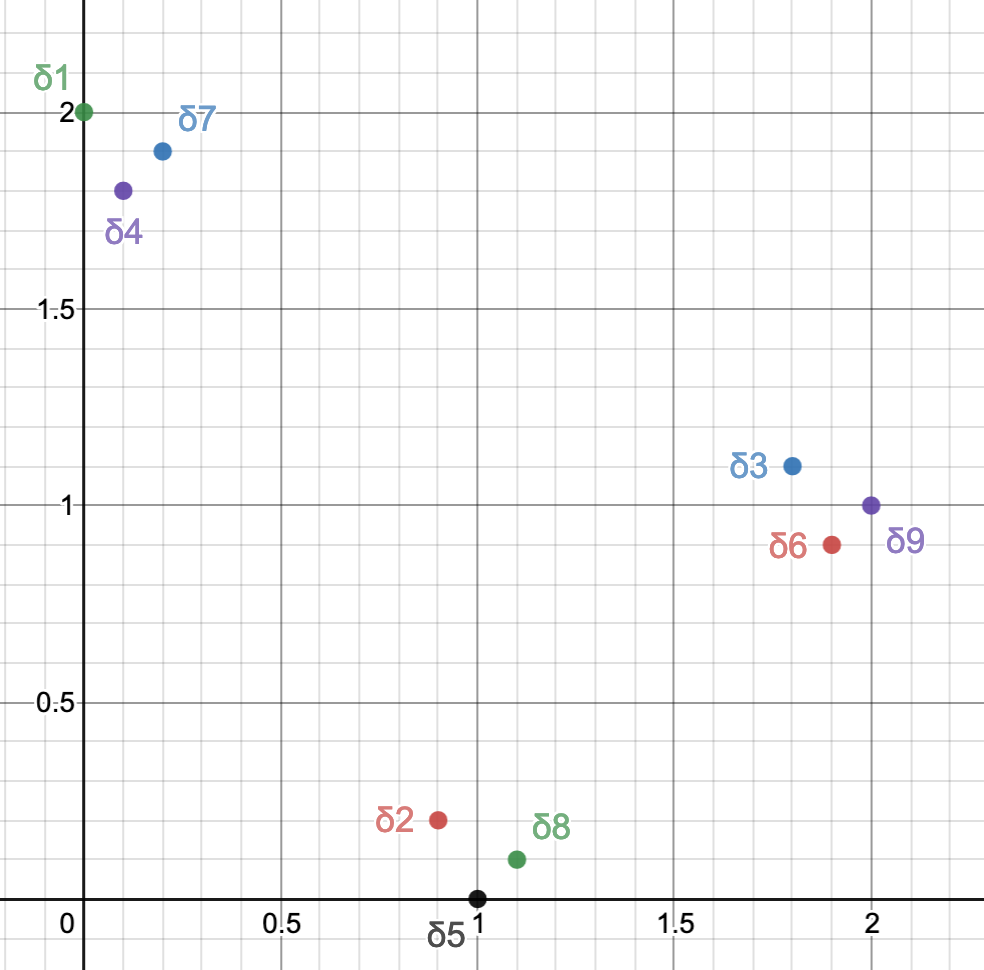
\includegraphics[height=.4\textheight]{minqi_s_solutions_to_the_problems_of_peter_j_bickel_and_kjell_a_doksum_2015_mathematical_statistics_basic_ideas_and_selected_topics_volume_1_2nd_edition_1.png}
\end{center}
\end{figure}
\item See below.\[
\begin{split}
R(\theta_1,\delta_1)&=1(0)+2(0)=0,\\
R(\theta_2,\delta_1)&=2(1)+1(0)=2,\\
R(\theta_1,\delta_2)&=1(1-p)+2(0)=0.9,\\
R(\theta_2,\delta_2)&=2(q)+1(0)=1.8,\\
R(\theta_1,\delta_3)&=1(0)+2(1-p)=1.8,\\
R(\theta_2,\delta_3)&=2(q)+1(1-q)=1.9,\\
R(\theta_1,\delta_4)&=1(p)+2(0)=0.1,\\
R(\theta_2,\delta_4)&=2(1-q)+1(0)=0.2,\\
R(\theta_1,\delta_5)&=1(1)+2(0)=1,\\
R(\theta_2,\delta_5)&=2(0)+1(0)=0,\\
R(\theta_1,\delta_6)&=1(p)+2(1-p)=1.9,\\
R(\theta_2,\delta_6)&=2(0)+1(1-q)=0.1,\\
R(\theta_1,\delta_7)&=1(0)+2(p)=0.2,\\
R(\theta_2,\delta_7)&=2(1-q)+1(q)=1.1,\\
R(\theta_1,\delta_8)&=1(1-p)+2(p)=1.1,\\
R(\theta_2,\delta_8)&=2(0)+1(q)=0.9,\\
R(\theta_1,\delta_9)&=1(0)+2(1)=2,\\
R(\theta_2,\delta_9)&=2(0)+1(1)=1.
\end{split}
\]
\begin{figure}[ht]
\begin{center}
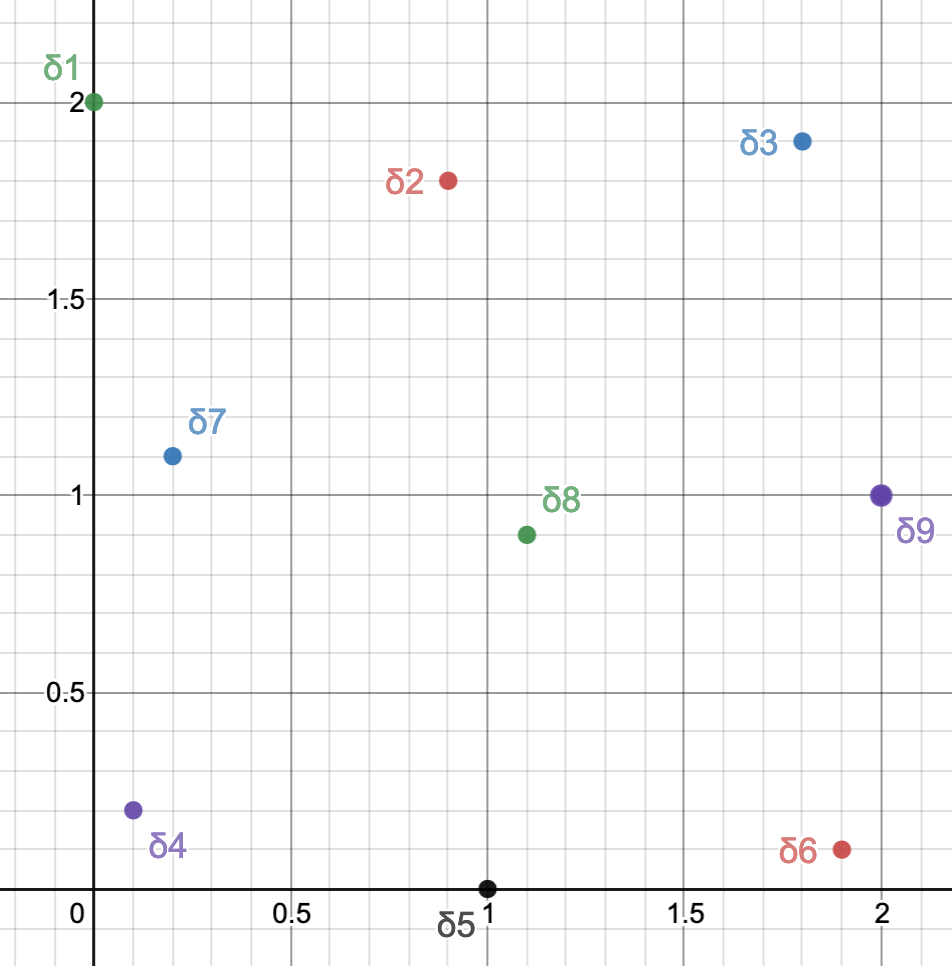
\includegraphics[height=.4\textheight]{minqi_s_solutions_to_the_problems_of_peter_j_bickel_and_kjell_a_doksum_2015_mathematical_statistics_basic_ideas_and_selected_topics_volume_1_2nd_edition_2.png}
\end{center}
\end{figure}
\end{enumerate}
\end{proof}

\section{Problem 1.4.1: Best Predictor, Best Linear Predictor, Best Zero Intercept LP}
An urn contains four red and four black balls. Four balls are drawn at random without replacement. Let $Z$ be the number of red balls obtained in the first two draws and $Y$ the total number of red balls drawn.
\begin{enumerate}[label=(\alph*)]
\item Find the best predictor of $Y$ given $Z$, the best linear predictor, and the best zero intercept linear predictor.
\item Compute the MSPEs of the predictors in (a).
\end{enumerate}
\begin{proof}[Answer]
\begin{enumerate}[label=(\alph*)]
\item Let $p(z,y)=P(Z = z,Y = y)$ be the joint probability mass function of $Z$ and $Y$, which is given by the following table.\[
\begin{array}{c|c|c|c|c|c}
z\backslash y&0&1&2&3&4\\\hline
0&1/16&2/16&1/16&0/16&0/16\\\hline
1&0/16&2/16&4/16&2/16&0/16\\\hline
2&0/16&0/16&1/16&2/16&1/16
\end{array}
\]We find\[
\begin{split}
E(Y|Z=0)&=\frac{16}{4}(1\cdot\frac{2}{16}+2\cdot\frac{1}{16}+3\cdot\frac{0}{16}+4\cdot\frac{0}{16})=1,\\
E(Y|Z=1)&=\frac{16}{8}(1\cdot\frac{2}{16}+2\cdot\frac{4}{16}+3\cdot\frac{2}{16}+4\cdot\frac{0}{16})=2,\\
E(Y|Z=2)&=\frac{16}{4}(1\cdot\frac{0}{16}+2\cdot\frac{1}{16}+3\cdot\frac{2}{16}+4\cdot\frac{1}{16})=3,\\
E(Z^2)&=1\cdot\frac{8}{16}+4\cdot\frac{4}{16}=\frac{24}{16},\\
E(Y^2)&=1\cdot\frac{4}{16}+4\cdot\frac{6}{16}+9\cdot\frac{4}{16}+16\cdot\frac{1}{16}=\frac{80}{16},\\
E(ZY)&=1\cdot\frac{2}{16}+2\cdot\frac{4}{16}+3\cdot\frac{2}{16}+4\cdot\frac{1}{16}+6\cdot\frac{2}{16}+8\cdot\frac{1}{16}=\frac{40}{16},\\
E(Z)&=1\cdot\frac{8}{16}+2\cdot\frac{4}{16}=\frac{16}{16},\\
E(Y)&=1\cdot\frac{4}{16}+2\cdot\frac{6}{16}+3\cdot\frac{4}{16}+4\cdot\frac{1}{16}=\frac{32}{16},\\
\text{Cov}(Z,Y)&=E(ZY)-E(Z)E(Y)=\frac{40}{16}-\frac{16}{16}\cdot\frac{32}{16}=\frac{1}{2},\\
\text{Var }Z&=E(Z^2)-(E(Z))^2=\frac{24}{16}-(\frac{16}{16})^2=\frac{1}{2}.
\end{split}
\]By Theorem~1.4.1 of \cite{bickel2015mathematical}, the following function $\mu_1$ is the best predictor:\[
\mu_1(z)\equiv E(Y|Z=z).
\]By Theorem~1.4.3 of \cite{bickel2015mathematical}, the following functions $\mu_2,\mu_3$ are the best linear predictor and the best zero intercept linear predictor, respectively:\[
\begin{split}
\mu_2(z)&\equiv a_1+b_1z,\\
\mu_3(z)&\equiv b_0z,
\end{split}
\]where\[
\begin{split}
b_0&\equiv\frac{E(ZY)}{E(Z^2)}=\frac{5}{3},\\
b_1&\equiv\frac{\text{Cov}(Z,Y)}{\text{Var }Z}=1,\\
a_1&\equiv E(Y)-b_1E(Z)=1.
\end{split}
\]
\item See below.\[
\begin{split}
E[\mu_1(Z)-Y]^2&=1\cdot\frac{1}{16}+1\cdot\frac{1}{16}+1\cdot\frac{2}{16}+1\cdot\frac{2}{16}+1\cdot\frac{1}{16}+1\cdot\frac{1}{16}\\
&=\frac{1}{2}=0.5,\\
E[\mu_2(Z)-Y]^2&=E[\mu_1(Z)-Y]^2\\
&=\frac{1}{2}=0.5,\\
E[\mu_3(Z)-Y]^2&=\left(0-0\right)^2\cdot\frac{1}{16}+\left(1-0\right)^2\cdot\frac{2}{16}+\left(2-0\right)^2\cdot\frac{1}{16}\\
&+\left(1-\frac{5}{3}\right)^2\cdot\frac{2}{16}+\left(2-\frac{5}{3}\right)^2\cdot\frac{4}{16}+\left(3-\frac{5}{3}\right)^2\cdot\frac{2}{16}\\
&+\left(2-\frac{10}{3}\right)^2\cdot\frac{1}{16}+\left(3-\frac{10}{3}\right)^2\cdot\frac{2}{16}+\left(4-\frac{10}{3}\right)^2\cdot\frac{1}{16}\\
&= \frac{43}{48}\approx 0.90.
\end{split}
\]
\end{enumerate}
\end{proof}

\section{Problem 1.5.1: Prove Sufficiency Directly and by the Factorization Theorem}
Let $X_1,\dots,X_n$ be a sample from a Poisson, $\mathcal{P}(\theta)$, population where $\theta>0$.
\begin{enumerate}[label=(\alph*)]
\item Show directly that $\sum_{i=1}^nX_i$ is sufficient for $\theta$.
\item Establish the same result using the factorization theorem.
\end{enumerate}
\begin{proof}
\begin{enumerate}[label=(\alph*)]
\item Define\[
\begin{split}
\mathbf{X}&\equiv(X_1,\dots,X_n)\\
T(\mathbf{X})&\equiv\sum_{i=1}^nX_i
\end{split}
\]Then\[
\begin{split}
P(\mathbf{X}=(x_1,\dots,x_n)|T(\mathbf{X})=t)&=\frac{P(\mathbf{X}=(x_1,\dots,x_n),T(\mathbf{X})=t)}{P(T(\mathbf{X})=t)}\\
&=\frac{\frac{\theta^{x_1}e^{-\theta}}{x_1!}\cdot\dots\cdot\frac{\theta^{x_n}e^{-\theta}}{x_n!}}{\frac{(n\theta)^te^{-n\theta}}{t!}}\\
&=\frac{\theta^te^{-n\theta}}{x_1!\cdot\dots\cdot x_n!}\cdot\frac{t!}{(n\theta)^te^{-n\theta}}\\
&=\frac{1}{x_1!\cdot\dots\cdot x_n!}\cdot\frac{t!}{n^t}\\
\end{split}
\]We have shown that $P(\mathbf{X}=(x_1,\dots,x_n)|T(\mathbf{X})=t)$ does not involve $\theta$. Hence, by definition, $T(\mathbf{X})$ is sufficient for $\theta$.
\item Define\[
\begin{split}
g(T(x_1,\dots,x_n),\theta)&\equiv\theta^{T(x_1,\dots,x_n)}e^{-n\theta},\\
h(x_1,\dots,x_n)&\equiv\frac{1}{x_1!\dots x_n!}.
\end{split}
\]Then\[
\begin{split}
P(\mathbf{X}=(x_1,\dots,x_n))&=\frac{\theta^{x_1}e^{-\theta}}{x_1!}\cdot\dots\cdot\frac{\theta^{x_n}e^{-\theta}}{x_n!}\\
&=\frac{\theta^te^{-n\theta}}{x_1!\cdot\dots\cdot x_n!}\\
&=g(T(x_1,\dots,x_n),\theta)\cdot h(x_1,\dots,x_n).
\end{split}
\]Theorem~1.5.1 of \cite{bickel2015mathematical} then implies that $T(\mathbf{X})$ is sufficient for $\theta$.
\end{enumerate}
\end{proof}

\section{Problem 1.6.1: $\mathcal{N}(\mu,\sigma^2),\Gamma(p,\lambda),\beta(r,s)$ Form $1$-parameter Exponential Families}
Prove the assertions of Table~1.6.1 of \cite{bickel2015mathematical}.
\begin{proof}
\begin{enumerate}
\item Suppose $p(x,\theta)$ is the density function of $\mathcal{N}(\theta,\sigma^2)$ where $\sigma^2$ is fixed, then\[
\begin{split}
p(x,\theta)&=\frac{1}{\theta\sqrt{2\pi}}\exp\left(-\frac{1}{2}\left(\frac{x-\theta}{\sigma}\right)^2\right)\\
&=\exp\left(\log\left(\frac{1}{\theta\sqrt{2\pi}}\right)\right)\exp\left(-\frac{1}{2}\left(\frac{x^2-2x\theta+\theta^2}{\sigma^2}\right)\right)\\
&=\exp\left(-\log(\theta\sqrt{2\pi})-\frac{x^2}{2\sigma^2}+\frac{x\theta}{\sigma^2}-\frac{\theta^2}{2\sigma^2}\right)\\
&=\exp\left(-\frac{x^2}{2\sigma^2}\right)\exp\left(-\log(\theta\sqrt{2\pi})+\frac{x\theta}{\sigma^2}-\frac{\theta^2}{2\sigma^2}\right).
\end{split}
\]Hence $\mathcal{N}(\theta,\sigma^2)$ form a one-parameter exponential family with\[
q=1,\eta(\theta)=\frac{\theta}{\sigma^2},B(\theta)=\log(\theta\sqrt{2\pi})+\frac{\theta^2}{2\sigma^2},T(x)=x,h(x)=\exp\left(-\frac{x^2}{2\sigma^2}\right).
\]Instead, suppose $p(x,\theta)$ is the density function of $\mathcal{N}(\mu,\theta^2)$ where $\mu$ is fixed, then\[
p(x,\theta)=\frac{1}{\mu\sqrt{2\pi}}\exp\left(-\frac{1}{2}\left(\frac{x-\mu}{\theta}\right)^2\right).
\]Hence $\mathcal{N}(\mu,\theta^2)$ form a one-parameter exponential family with\[
q=1,\eta(\theta)=-\frac{1}{2\theta^2},B(\theta)=0,T(x)=(x-\mu)^2,h(x)=\frac{1}{\mu\sqrt{2\pi}}.
\]
\item Suppose $p(x,\theta)$ is the density function of $\Gamma(p,\theta)$ where $p$ is fixed, then\[
\begin{split}
p(x,\theta)&=\frac{\theta^px^{p-1}e^{-\theta x}}{\Gamma(p)}\\
&=\frac{x^{p-1}}{\Gamma(p)}\exp(\log(\theta^p)-\theta x)\\
\end{split}
\]Hence $\Gamma(p,\theta)$ form a one-parameter exponential family with\[
q=1,\eta(\theta)=-\theta,B(\theta)=-\log(\theta^p),T(x)=x,h(x)=\frac{x^{p-1}}{\Gamma(p)}.
\]Instead, suppose $p(x,\theta)$ is the density function of $\Gamma(\theta,\lambda)$ where $\lambda$ is fixed, then\[
\begin{split}
p(x,\theta)&=\frac{\lambda^\theta x^{\theta-1}}{\Gamma(p)}\\
&=\frac{e^{-\lambda x}}{\Gamma(p)}\exp(\log(\lambda^\theta)+(\theta-1)\log(x))\\
\end{split}
\]Hence $\Gamma(\theta,\lambda)$ form a one-parameter exponential family with\[
q=1,\eta(\theta)=\theta-1,B(\theta)=-\log(\lambda^\theta),T(x)=\log(x),h(x)=\frac{e^{-\lambda x}}{\Gamma(p)}.
\]
\item Suppose $p(x,\theta)$ is the density function of $\beta(r,\theta)$ where $r$ is fixed, then\[
\begin{split}
p(x,\theta)&=\frac{\Gamma(r+\theta)x^{r-1}(1-x)^{\theta-1}}{\Gamma(r)\Gamma(\theta)}\\
&=\frac{x^{r-1}}{\Gamma(r)}\cdot\frac{\Gamma(r+\theta)(1-x)^{\theta-1}}{\Gamma(\theta)}\\
&=\frac{x^{r-1}}{\Gamma(r)}\cdot\exp(\log(\Gamma(r+\theta))+(\theta-1)\log(1-x)-\log(\Gamma(\theta)))
\end{split}
\]Hence $\beta(r,\theta)$ form a one-parameter exponential family with\[
q=1,\eta(\theta)=\theta-1,B(\theta)=\log(\Gamma(\theta))-\log(\Gamma(r+\theta)),T(x)=\log(1-x),h(x)=\frac{x^{r-1}}{\Gamma(r)}.
\]Instead, suppose $p(x,\theta)$ is the density function of $\beta(\theta,s)$ where $s$ is fixed, then\[
\begin{split}
p(x,\theta)&=\frac{\Gamma({\theta+s})x^{\theta-1}(1-x)^{s-1}}{\Gamma(\theta)\Gamma(s)}\\
&=\frac{(1-x)^{s-1}}{\Gamma(s)}\cdot\frac{\Gamma({\theta+s})x^{\theta-1}}{\Gamma(\theta)}\\
&=\frac{(1-x)^{s-1}}{\Gamma(s)}\cdot\exp(\log(\Gamma(\theta+s))+(\theta-1)\log(x)-\log(\Gamma(\theta)))
\end{split}
\]Hence $\beta(\theta,s)$ form a one-parameter exponential family with\[
q=1,\eta(\theta)=\theta-1,B(\theta)=\log(\Gamma(\theta))-\log(\Gamma(\theta+s)),T(x)=\log(x),h(x)=\frac{(1-x)^{s-1}}{\Gamma(s)}.
\]
\end{enumerate}
\end{proof}

\backmatter
\bibliographystyle{amsalpha}
\bibliography{../../bibliography.bib}
\end{document}
